\begin{figure}
    \begin{center}
        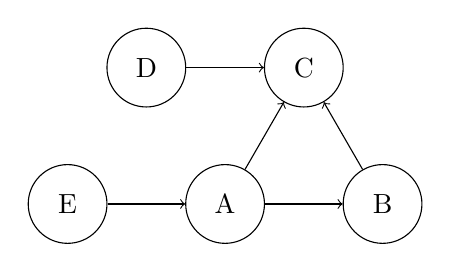
\begin{tikzpicture}
            % Define vertices
            \node[circle,draw,minimum size=1cm] (A) at (0,0) {A};
            \node[circle,draw,minimum size=1cm] (B) at (2,0) {B};
            \node[circle,draw,minimum size=1cm] (C) at (1,1.732) {C};
            \node[circle,draw,minimum size=1cm] (D) at (-1,1.732) {D};
            \node[circle,draw,minimum size=1cm] (E) at (-2,0) {E};
            
            % Draw edges
            \draw[->](A) -- (B);
            \draw[->](B) -- (C);
            \draw[->](D) -- (C);
            \draw[->](E) -- (A);
            \draw[->](A) -- (C);
            \end{tikzpicture}
        \caption{Example graph with five nodes and five edges}
        \label{figure:graph-example}          
    \end{center}
\end{figure}